\documentclass[../report/main.tex]{subfiles}
 
\begin{document}

\begin{enumerate}[a)]
	\item What are the lengths of the shortest paths from vertex $a$ to all other vertices?

    The shortest path problem can be solved using a linear programming model of the following form:

    maximize $d_t$
    subject to $d_s = 0$
               $d_v - d_u \leq l_{u -> v}$ for every edge $u$ -> $v$

    Based on the paths and weights denoted from the Project3Problem3-1.txt file the expressions for the linear programming solution to find shortest paths will be:

    \begin{itemize}
      \item $d_b - d_a \leq 2$
      \item $d_c - d_a \leq 3$
      \item $d_d - d_a \leq 8$
      \item $d_h - d_a \leq 9$
      \item $d_a - d_b \leq 4$
      \item $d_c - d_b \leq 5$
      \item $d_e - d_b \leq 7$
      \item $d_f - d_b \leq 4$
      \item $d_d - d_c \leq 10$
      \item $d_b - d_c \leq 5$
      \item $d_g - d_c \leq 9$
      \item $d_i - d_c \leq 11$
      \item $d_f - d_c \leq 4$
      \item $d_a - d_d \leq 8$
      \item $d_g - d_d \leq 2$
      \item $d_j - d_d \leq 5$
      \item $d_f - d_d \leq 1$
      \item $d_h - d_e \leq 5$
      \item $d_c - d_e \leq 4$
      \item $d_i - d_e \leq 10$
      \item $d_i - d_f \leq 2$
      \item $d_g - d_f \leq 2$
      \item $d_d - d_g \leq 2$
      \item $d_j - d_g \leq 8$
      \item $d_k - d_g \leq 12$
      \item $d_i - d_h \leq 5$
      \item $d_k - d_h \leq 10$
      \item $d_a - d_i \leq 20$
      \item $d_k - d_i \leq 6$
      \item $d_j - d_i \leq 2$
      \item $d_m - d_i \leq 12$
      \item $d_i - d_j \leq 2$
      \item $d_k - d_j \leq 4$
      \item $d_l - d_j \leq 5$
      \item $d_h - d_k \leq 10$
      \item $d_m - d_k \leq 10$
      \item $d_m - d_l \leq 2$
    \end{itemize}

    An image of the graph is below:

    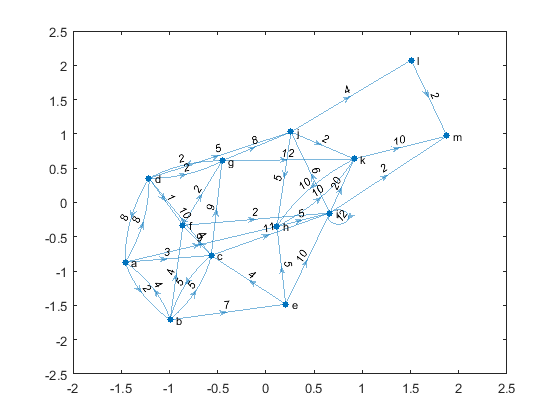
\includegraphics{../problem_three/img/problem3_digraph.png}

    Code used to find the shortest paths:
  
    \lstinputlisting{../problem_three/matlab/problem3_partA.m}

    The lengths of the shortest paths from a to the other vertices in the graph are listed below:
    
    \lstinputlisting{../problem_three/matlab/P3A_solution.txt}

	\item If a vertex $z$ is added to the graph for which there is no path from vertex $a$ to vertex $z$, what will be the result when you attempt to find the lengths of shortest paths as in part a).

    Graphic with the new vertex z added:

    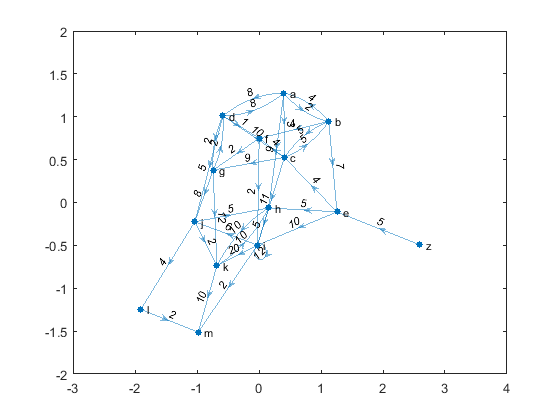
\includegraphics{../problem_three/img/problem3_digraph_with_z.png}

    \lstinputlisting{../problem_three/matlab/problem3_partB.m}

    When using the script above with the new vertex z the matlab code fails with this message: "Exiting: One or more of the residuals, duality gap, or total relative error
has stalled:
        the dual appears to be infeasible and the primal unbounded since
        the primal objective < -1e+10
        and the dual objective < 1e+6."

    This error is consistent with what is expected because we are trying to find the shortest path from a to all other vertices however that is not feasible with the new vertex z because we made it inaccessible.

    However a workaround for this result would be to look at the preliminary optimization results to see which nodes are causing problems. We can specify those problem nodes to fixed dummy distances that are very large relative to the longest feasible path(s). We then rerun the script to obtain the shortest paths for the remaining reachable nodes.

	\item What are the lengths of the shortest paths from each vertex to vertex $m$? How can you solve this problem with just one linear program?
    
    For this part we just swapped the directionality on all the edges from part A and set the origin to be vertex m. This yields the distance from m to every other vertex at once which the distances would be equivalent regardless of direction so it works out.

    Code used to find the shortest paths from all other vertices using a single linear program:

    \lstinputlisting{../problem_three/matlab/problem3_partC.m}

    Output of the paths after running the above script:

    \lstinputlisting{../problem_three/matlab/P3C_solution.txt}

	\item Suppose that all paths must pass through vertex $i$. How can you calculate the length of the shortest path from any vertex $x$ to vertex $y$ that pass through vertex $i$ (for all $x, y \in V$)? Calculate the lengths of these paths for the given graph. (Note: for some vertices $x$ and $y$, it may be impossible to pass through vertex $i$).

    Code used to find the paths from one vertex to another while passing through an intermediate vertex $i$:

    \lstinputlisting{../problem_three/matlab/problem3_partD.m}

    The outputted paths after running the above script:

    \lstinputlisting{../problem_three/matlab/P3D_solution.txt}
\end{enumerate}

\end{document}
